\textbf{Luke Wiskus:}
A large lesson that we learned was that it is important to divide the work of the project into more manageable classes. Our original implementation did not use a Color class and instead just manipulated the pixels directly from the image char array whenever it was necessary. This is an alternate approach that works when implemented correctly, but has its own drawbacks. \\ 

While you're spared the time of designing and creating a Color class, you pay for it down the line with less readable code, making it harder to debug and make changes when solving problems. We realized quickly that scaling this was a lot more difficult than creating a Color class, so that was a major discovery that made our code base much more manageable when we switched over. A lesson learned would be that a little effort spent planning upfront can save you a lot of headache down the line. \\
	
\textbf{Fletcher Gornick:}
Our original design that we altered a bit to give us our finished product contained the Image Processor class which we ultimately decided to drop.  Depending on how our next two iterations go, we may bring it back though. The UML diagram below shows this, as well as our original intentions for how our filters would interact with our Simple and Convolution filters.

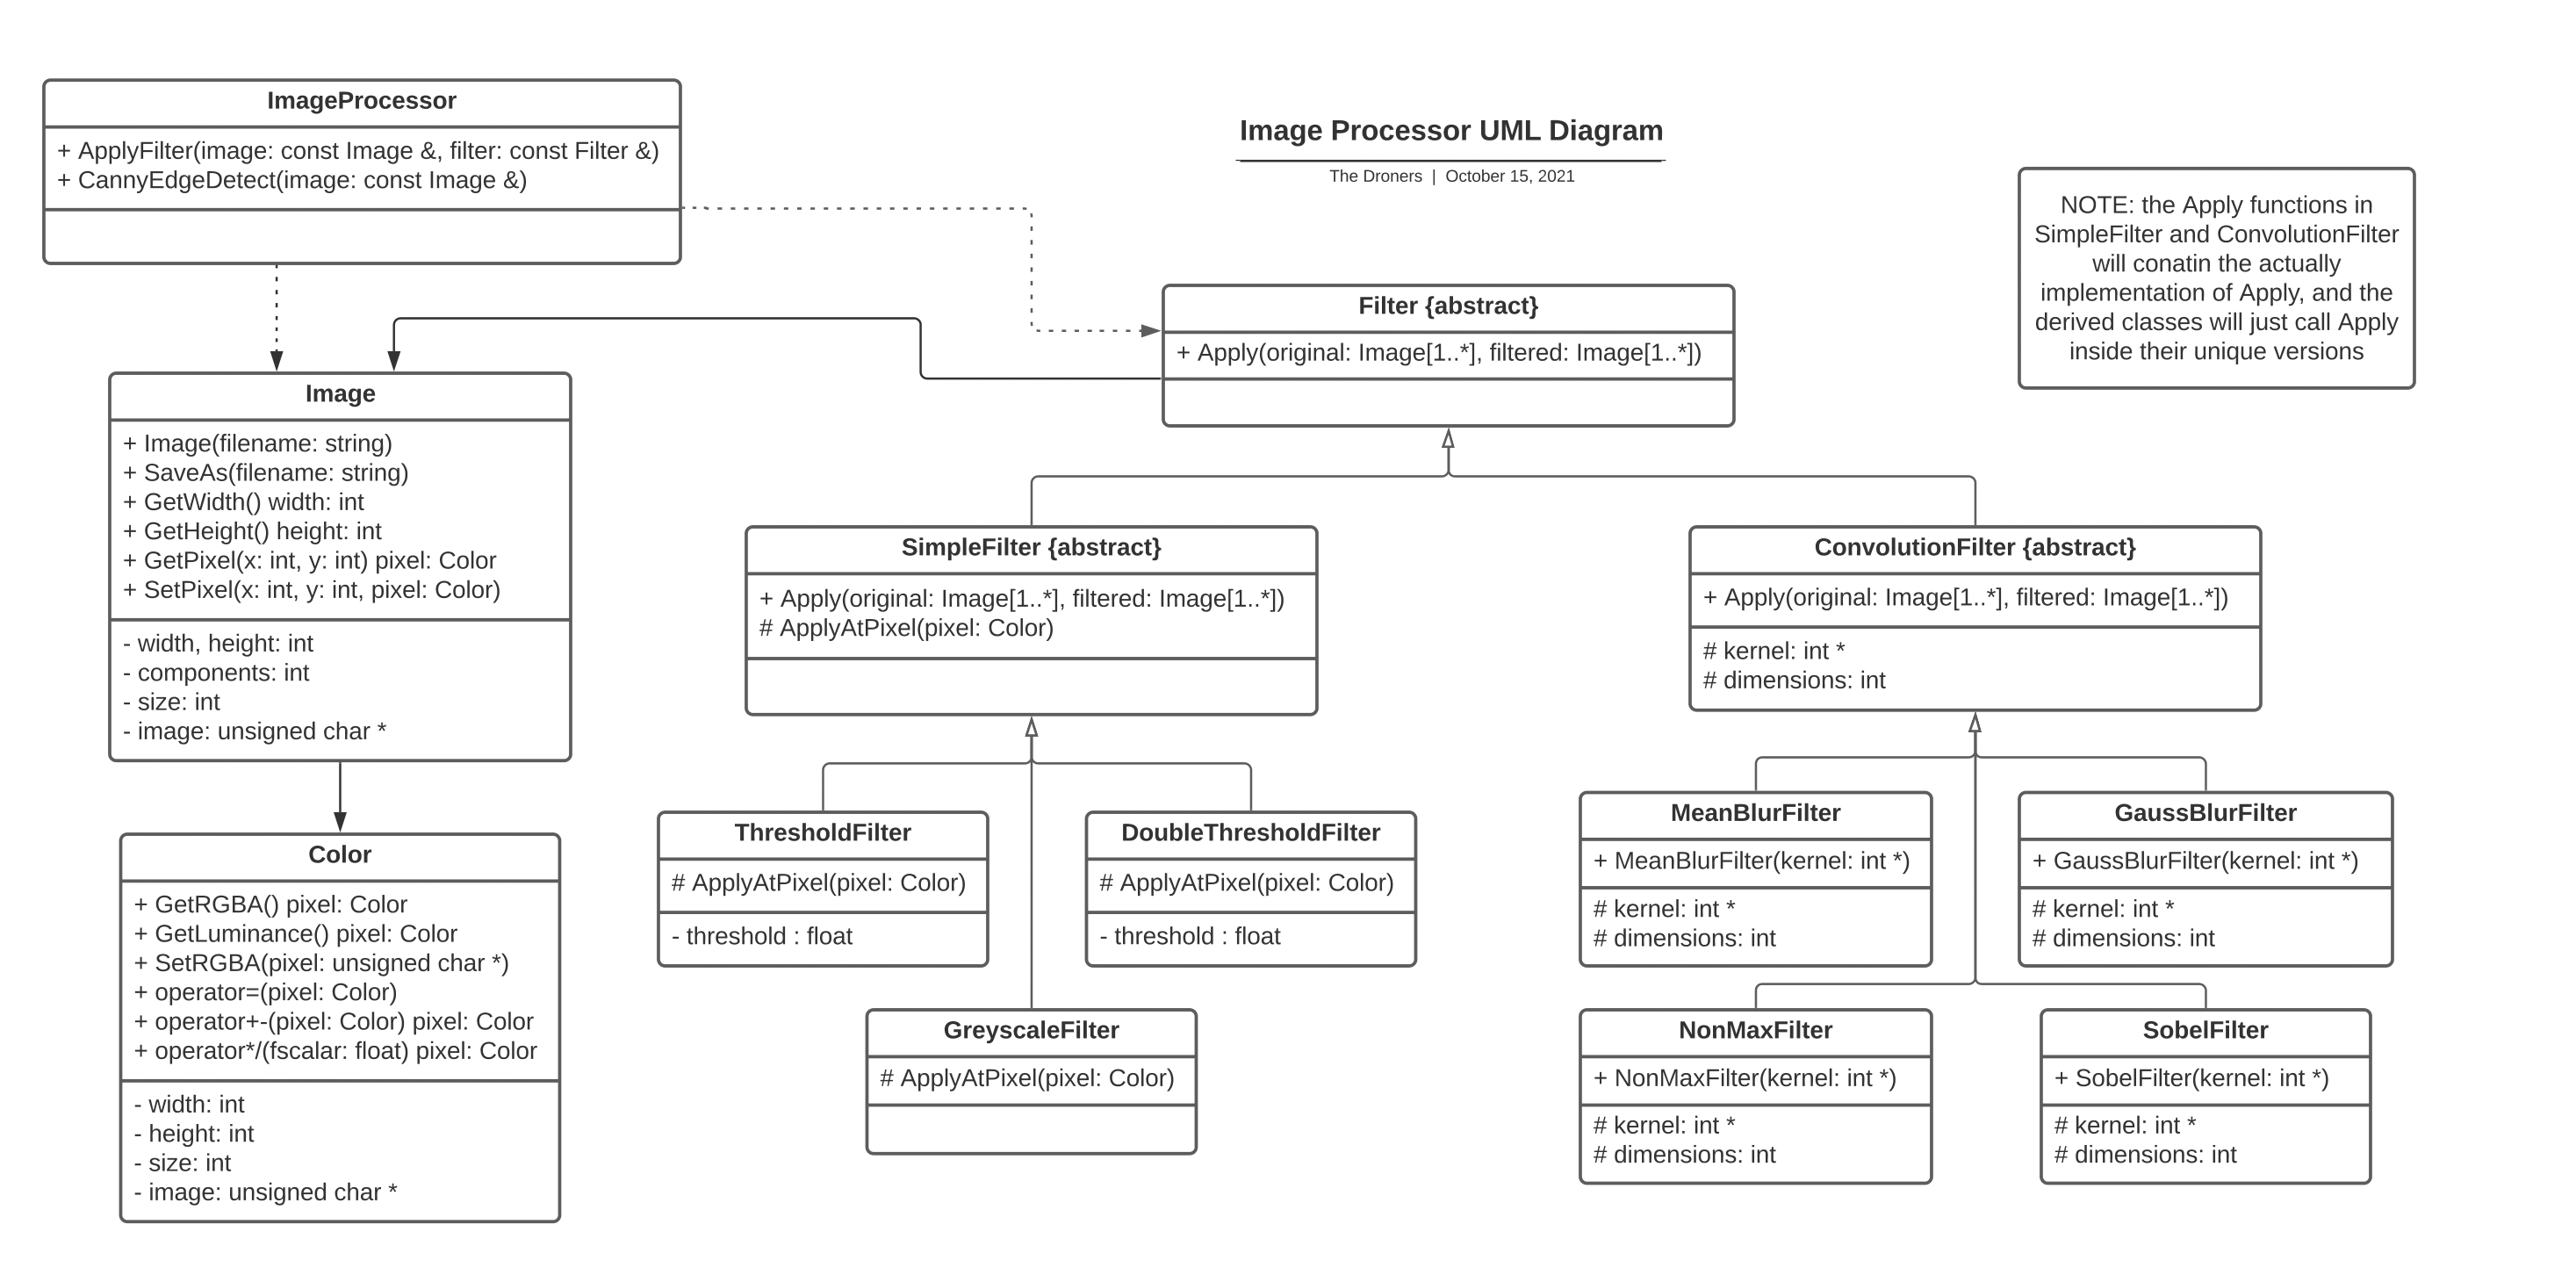
\includegraphics[width=\textwidth]{original.png}

Our current Convolution Filter class allows for kernels of different sizes, with flexible code that seamlessly integrates the different kernel sizes. An alternative design choice would've been to define a standardized 3x3 kernel, which wouldn't be as extensible or flexible as our current design. We also thought about using a couple different methods for our canny edge detector to see if they improve the performance \cite{canny}. Jason will go over some of these alternatives. \\

\textbf{Jason Woitalla:}
As stated above by Fletcher, it may be in our future interest to increase the rate at which we can convert images into their Canny-edge-detected states. If we want to be able to evaluate more than one image every few seconds it would do good to seek out areas where we can improve performance. One such of those cases might be the using the Laplacian method \cite{laplace}. \\

There are two generally classified ways to go about computing the Canny edge detection, the first of which is the gradient method that we're currently implementing. The other is the Laplacian, which computes the edges by looking for zeros in the second derivative of the image intensity. While we haven't implemented the filter this way yet, it is an alternate solution that may be worth looking into should our current gradient method of calculating prove inadequate. \newpage


\textbf{Gabe Fendrich:}
As stated previously, the current implementation of our project follows very closely along the OOP paradigm. We have a multitude of different header files and three separate interfaces, along with lots of Inheritance and Polymorphism going on. An alternate approach could have been implementing a functional style approach, forgoing the hierarchy of different classes and structures and compressing them down into a few files with tons of functions \cite{cravey}. \\

While technically possible this approach would be an absolute pain to work with in the context of this project. Working with OOP principles allows us to easily plot out the relationships between the programs with UML diagrams, and facilitates the expansion and maintenance of the program as time goes on. A functional approach would be much harder to scale and keep track of the moving parts. A lesson would be that it's better to evaluate what the needs of a project are going to be, and then choose a coding style whose strengths play to the task at hand. \\

\textbf{Peyton Johnson:}
We could have done naming differently e.g. instead of threshold\_filter we could have done something like thresh. If we didn't set up the naming for the .h and .cc files as we did it could get confusing later on as the scope of the project grows. This naming convention also allowed me to easily implement the filters for canny\_edge without having to actually look through all the files to find what someone had named their files. \\

The final design choice we made with an alternative that's worth going over is the header guard. The question on why we use the standard header guard as opposed to the \texttt{pragma} guard was brought to my attention by a piazza post \cite{tom}.  We thought it’d be an interesting choice to use the \texttt{pragma} method, but we decided against it considering \texttt{ifndef} has been the industry standard forever, but this alternative is certainly worth noting.


